%% It is just an empty TeX file.
%% Write your code here.
% !TEX encoding = UTF-8 Unicode
\documentclass[a4paper, 12pt]{article}   	% use "amsart" instead of "article" for AMSLaTeX format
\usepackage[left=20mm, top=15mm, right=10mm, bottom=15mm]{geometry}    

            
\usepackage[parfill]{parskip}    		% Activate to begin paragraphs with an empty line rather than an indent
\usepackage{graphicx}				% Use pdf, png, jpg, or eps§ with pdflatex; use eps in DVI mode
\usepackage[14pt]{extsizes}
\usepackage{setspace,amsmath}
\usepackage{mathtools}
\usepackage{graphicx}
\usepackage{ dsfont }
\usepackage{amsmath,amssymb}
\usepackage[unicode]{hyperref}

\usepackage{xcolor}
\usepackage{color}
\usepackage{minted}
\usepackage{caption}

\usepackage{array}
\newcolumntype{P}[1]{>{\centering\arraybackslash}p{#1}}

\usepackage{cmap} % Улучшенный поиск русских слов в полученном pdf-файле
\usepackage[T2A]{fontenc} % Поддержка русских букв
\usepackage[utf8]{inputenc} % Кодировка utf8
\usepackage[english, russian]{babel} % Языки: русский, английский

								% TeX will automatically convert eps --> pdf in pdflatex		
\usepackage{amssymb}

\begin{document}
\begin{titlepage}

\thispagestyle{empty}

\begin{center}
Федеральное государственное бюджетное образовательное учреждение высшего профессионального образования Московский государственный технический университет имени Н.Э. Баумана
\end{center}


\vfill

\centerline{\large{Лабораторная работа}}

\centerline{\large{«Решение баллистической задачи»}}

\centerline{\large{по курсу}}
\centerline{\large{«Моделирование»}}


\vfill

Студент группы ИУ9-82 \hfill Белогуров А.А.

Преподаватель \hfill Домрачева А.Б.
\vfill

\centerline{Москва, 2018}
\clearpage
\end{titlepage}

\newpage
\setcounter{page}{2}

\tableofcontents

\newpage

\section{Постановка задачи}
    Смоделировать полёт баллистического снаряда методом Ньютона с учётом коэффициента сопротивления воздуха. Сравнить полученные результаты для данного метода с коэффициентом равным нулю и методом Галилея.
    
    Даны следующие начальные данные: свинцовый шарик радиусом $r = 0.05$ м брошен под углом $\alpha = 30$ градусов с начальной скоростью $v_0 = 50$ м/с.
    

\newpage

\section{Теоретические сведения}
\subsection{Модель Ньютона}
    \begin{center}
        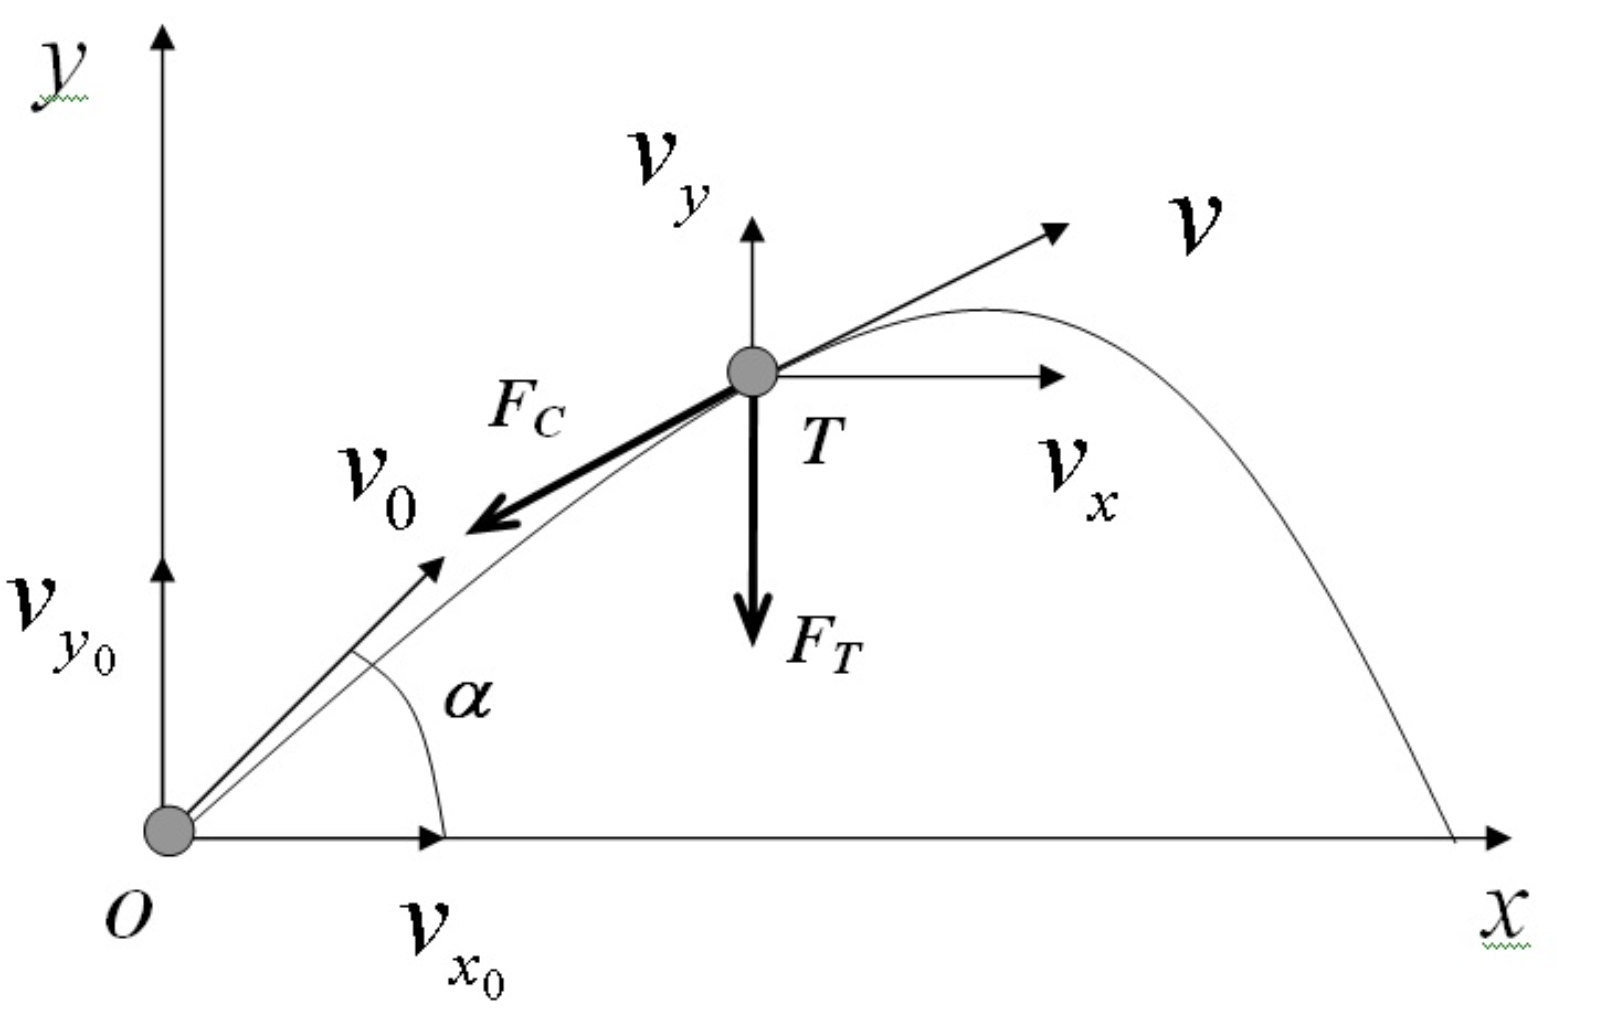
\includegraphics[height=5cm]{newton_model}
    \end{center}
    Главное отличие модели Ньютона от модели Галилея заключается в учитывании силы сопротивления воздуха $F_c = \beta v^2$, коэффициент которой вычисляется по формуле:
    \begin{equation}
        \beta = \frac{C \rho S}{2},
    \end{equation}
    где $C$ - коэффициент лобового сопротивления (для многих задач баллистики $C \approx 0.15$), $S$ – площадь поперечного сечения ($S = \pi r^2$), $\rho$ - плотность воздуха ($\rho=1,29$ кг/м$^3$). 
    
    При $\beta = 0$ модель Ньютона является частным случаем методом Галилея.
    
    Основной идеей данного метода является решений системы дифференциальных уравнений:
    
    \begin{equation}
        \begin{dcases*}
            \frac{dv_x}{dt} = - \frac{\beta v_x}{m} \sqrt{v_x^2 + v_y^2} \\
            \frac{dv_y}{dt} = - \frac{\beta v_y}{m} \sqrt{v_x^2 + v_y^2} - g \\
            \frac{dx}{dt} = v_x \\
            \frac{dy}{dt} = v_y
        \end{dcases*},
    \end{equation}
    при следующих начальных условиях:
    \begin{equation}
        \begin{dcases*}
            v_x(0) = v_0 cos(\alpha) \\
            v_y(0) = v_0 sin(\alpha) \\
            x(0) = 0 \\
            y(0) = 0
        \end{dcases*}.
    \end{equation}

    Для решения первой системы воспользуемся методом Рунге-Кутта 4-го порядка обеспечивающий достаточно высокую точность вычислений.
    
\subsection{Модель Галилея}
    Рисунок к модели Галилея будет идентичен модели Ньютона за исключением того, что не будет учтена сила сопротивления воздуха. Следовательно для вычисления конечной координаты $x$ воспользуемся формулой:
    \begin{equation}
        x = \frac{2 tan(\alpha) (cos(\alpha)v_0)^2}{g},
    \end{equation}
    где g - ускорение свободного падения.

\newpage

\section{Практическая реализация}
Далее приведена реализация программы на языке Python 3, которая вычисляет конечную координату x для метода Галилея и методов Ньютона с учётом коэффициента сопротивления и без его учёта \hyperlink{lst:Lab1}(Листинг 1).
 
\hypertarget{lst:Lab1}{}
\inputminted[frame=single,framesep=10pt, fontsize = \small, linenos=true, breaklines]{python}{Lab1.py}

\newpage
\section{Результаты}
    Для приведённых в первом разделе начальных условий были получены следующие значения:
    \begin{table}[h]
    \begin{center}
        \begin{tabular}{|P{5cm}|P{7cm}|}
            \hline
            Модель & Координата X \\
            \hline
            \multicolumn{2}{|c|} {$r = 0.05$ м, $\alpha = 30$, $v_0 = 50$ м/c}\\
            \hline
            Галилей & 220.69964  \\
            \hline
            Ньютон & 216.34459 \\
            \hline
            Ньютон $\beta = 0$ & 220.403465  \\
            \hline
        \end{tabular}
    \end{center}
    \end{table}
    
    Поменяем исходные данныe:
     \begin{table}[h]
    \begin{center}
        \begin{tabular}{|P{5cm}|P{7cm}|}
            \hline
            Модель & Координата X \\
            \hline
            \multicolumn{2}{|c|} {$r = 0.05$ м, $\alpha = 15$, $v_0 = 10$ м/c}\\
            \hline
            Галилей & 5.09683  \\
            \hline
            Ньютон & 5.02115 \\
            \hline
            Ньютон $\beta = 0$ & 5.022814  \\
            \hline
            \multicolumn{2}{|c|} {$r = 0.05$ м, $\alpha = 45$, $v_0 = 30$ м/c}\\
            \hline
            Галилей & 91.74311  \\
            \hline
            Ньютон & 90.81862 \\
            \hline
            Ньютон $\beta = 0$ & 91.64103  \\
            \hline
            \multicolumn{2}{|c|} {$r = 0.05$ м, $\alpha = 50$, $v_0 = 60$ м/c}\\
            \hline
            Галилей & 361.39734  \\
            \hline
            Ньютон & 347.99881 \\
            \hline
            Ньютон $\beta = 0$ & 361.37519  \\
            \hline
        \end{tabular}
    \end{center}
    \end{table}
    

\newpage
\section{Вывод}
    В ходе выполнения лабораторной работы были изучены модели Ньютона и Галилея для решения баллистической задачи и была написана их реализация на языке Python 3.
    
    Для решения системы дифференциальных уравнений в методе Ньютона использовался метод Рунге-Кутта 4-го порядка, который имеет четвёртый порядок точности, но стоит отметить, что так как все вычисления производились на ЭВМ, то конечный резульатат может отличаться от реального и иметь вычислительные погрешности.
    
    Так как модель Ньютона учитывает силу сопротивление воздуха, то точка падения снаряда должна быть ближе к точке запуска, что наглядно видно в предыдущем разделе. Если же ёе не учитывать и принимать коэффициент сопротивления воздуха $\beta = 0$, то точка падения близится к точке падения модели Галилея.



\end{document} 














